\documentclass[../en-fa-lab.tex]{subfiles}
\usepackage{hyperref}
\hypersetup{
    pdftitle={(EN) L9 - Tutorial},   % The title shown in the browser tab
    pdfauthor={},         % Your name or organization
    pdfsubject={},   % A brief description
    pdfkeywords={}
}

\begin{document}

\section{\texorpdfstring{\textbf{Assignment 9: Tutorial}}{Assignment 9: Tutorial}}\label{assign9}


\subsection{Visual Studio Project Setup}\label{visual-studio-project-setup}

\begin{enumerate}
\def\labelenumi{\arabic{enumi}.}
\item
  Go to moodle and select one of the following:
\end{enumerate}

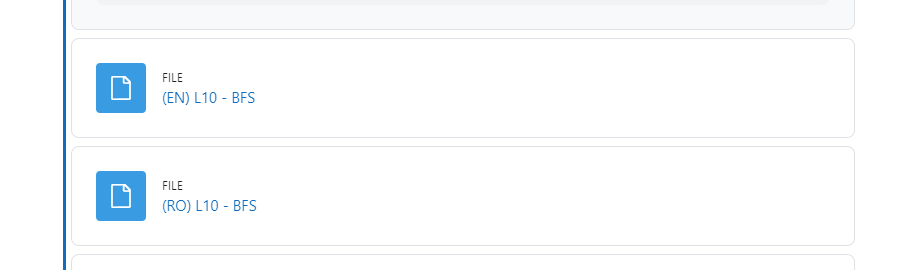
\includegraphics[width=\textwidth,alt={A white rectangular object with a black border Description automatically generated with medium confidence}]{./Resources/tutorial_lab9/image1.png}

This will result in a `.zip' file being downloaded.

\begin{enumerate}
\def\labelenumi{\arabic{enumi}.}
\setcounter{enumi}{1}
\item
  Create an Empty C++ Project and by right-clicking on the project (not
  the solution) you will be able to select `Open Folder in File
  Explorer'.
\end{enumerate}

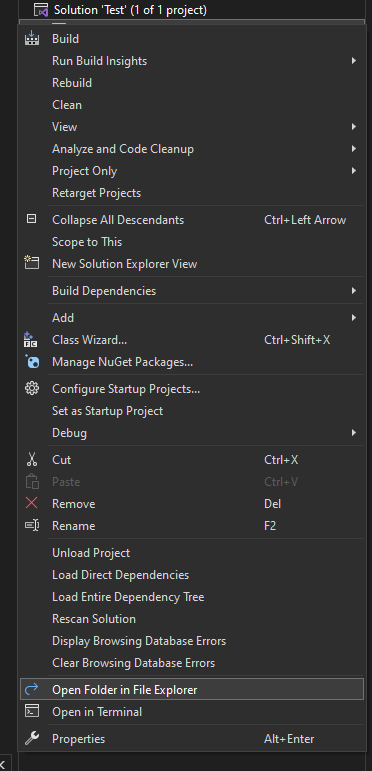
\includegraphics[width=\textwidth,alt={A screenshot of a computer Description automatically generated}]{./Resources/tutorial_lab9/image2.png}

\begin{enumerate}
\def\labelenumi{\arabic{enumi}.}
\setcounter{enumi}{2}
\item
  At this point, a `File Explorer' window will be opened. Open another
  `File Explorer' with the location of your downloads (most likely the
  Downloads folder).
\end{enumerate}

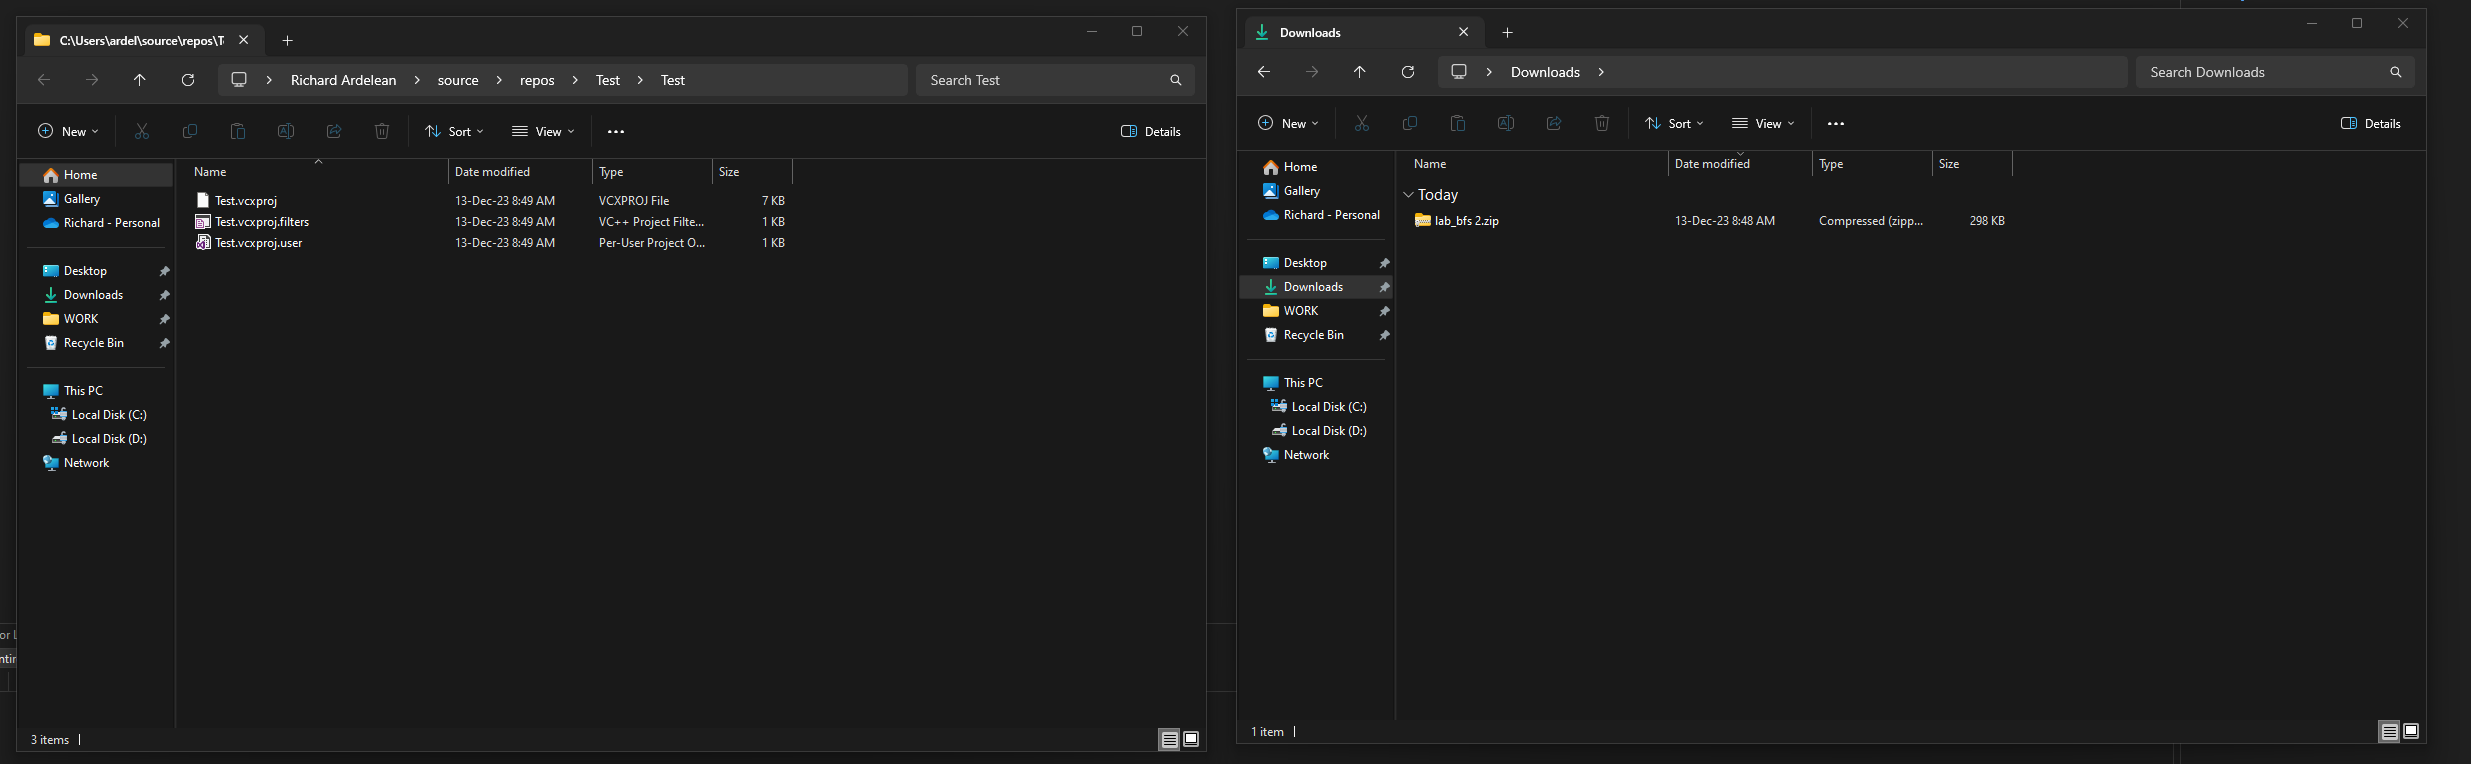
\includegraphics[width=\textwidth,alt={A screenshot of a computer Description automatically generated}]{./Resources/tutorial_lab9/image3.png}

\begin{enumerate}
\def\labelenumi{\arabic{enumi}.}
\setcounter{enumi}{3}
\item
  Open the `.zip' file and copy as shown below the files from the zip
  file to the folder of the project.
\end{enumerate}

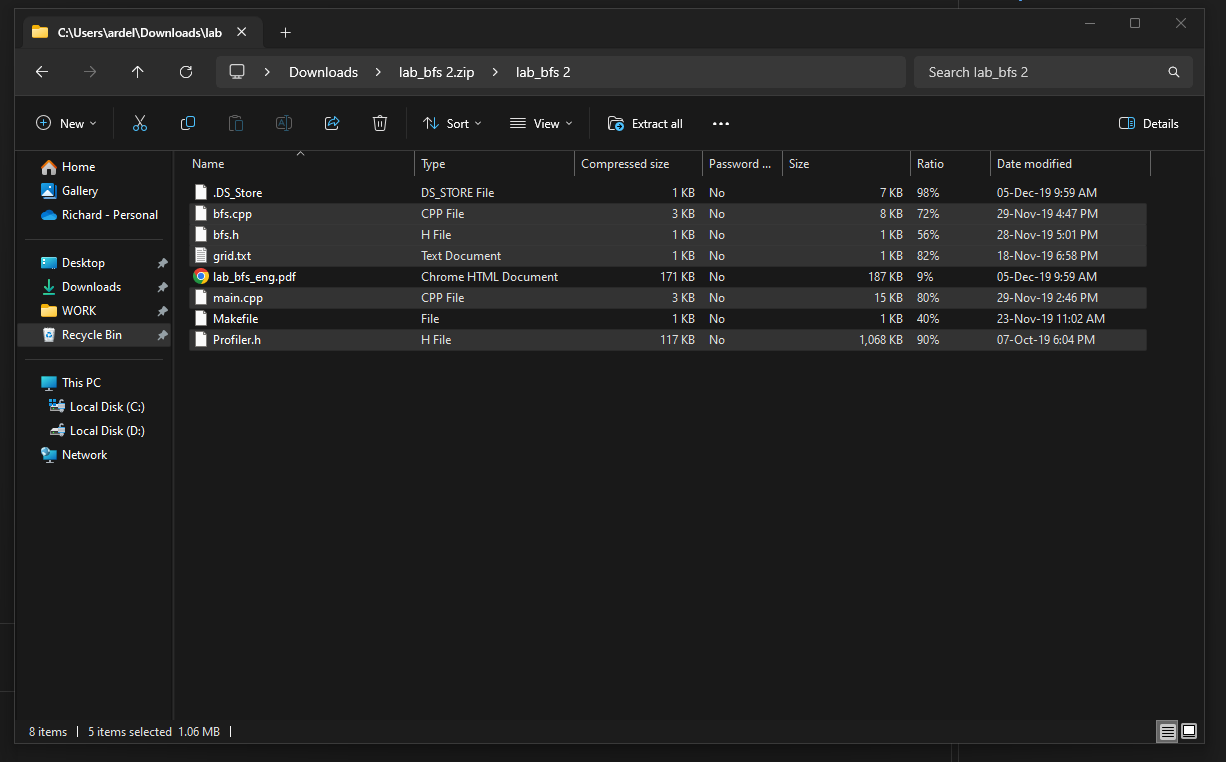
\includegraphics[width=\textwidth,alt={A screenshot of a computer Description automatically generated}]{./Resources/tutorial_lab9/image4.png}

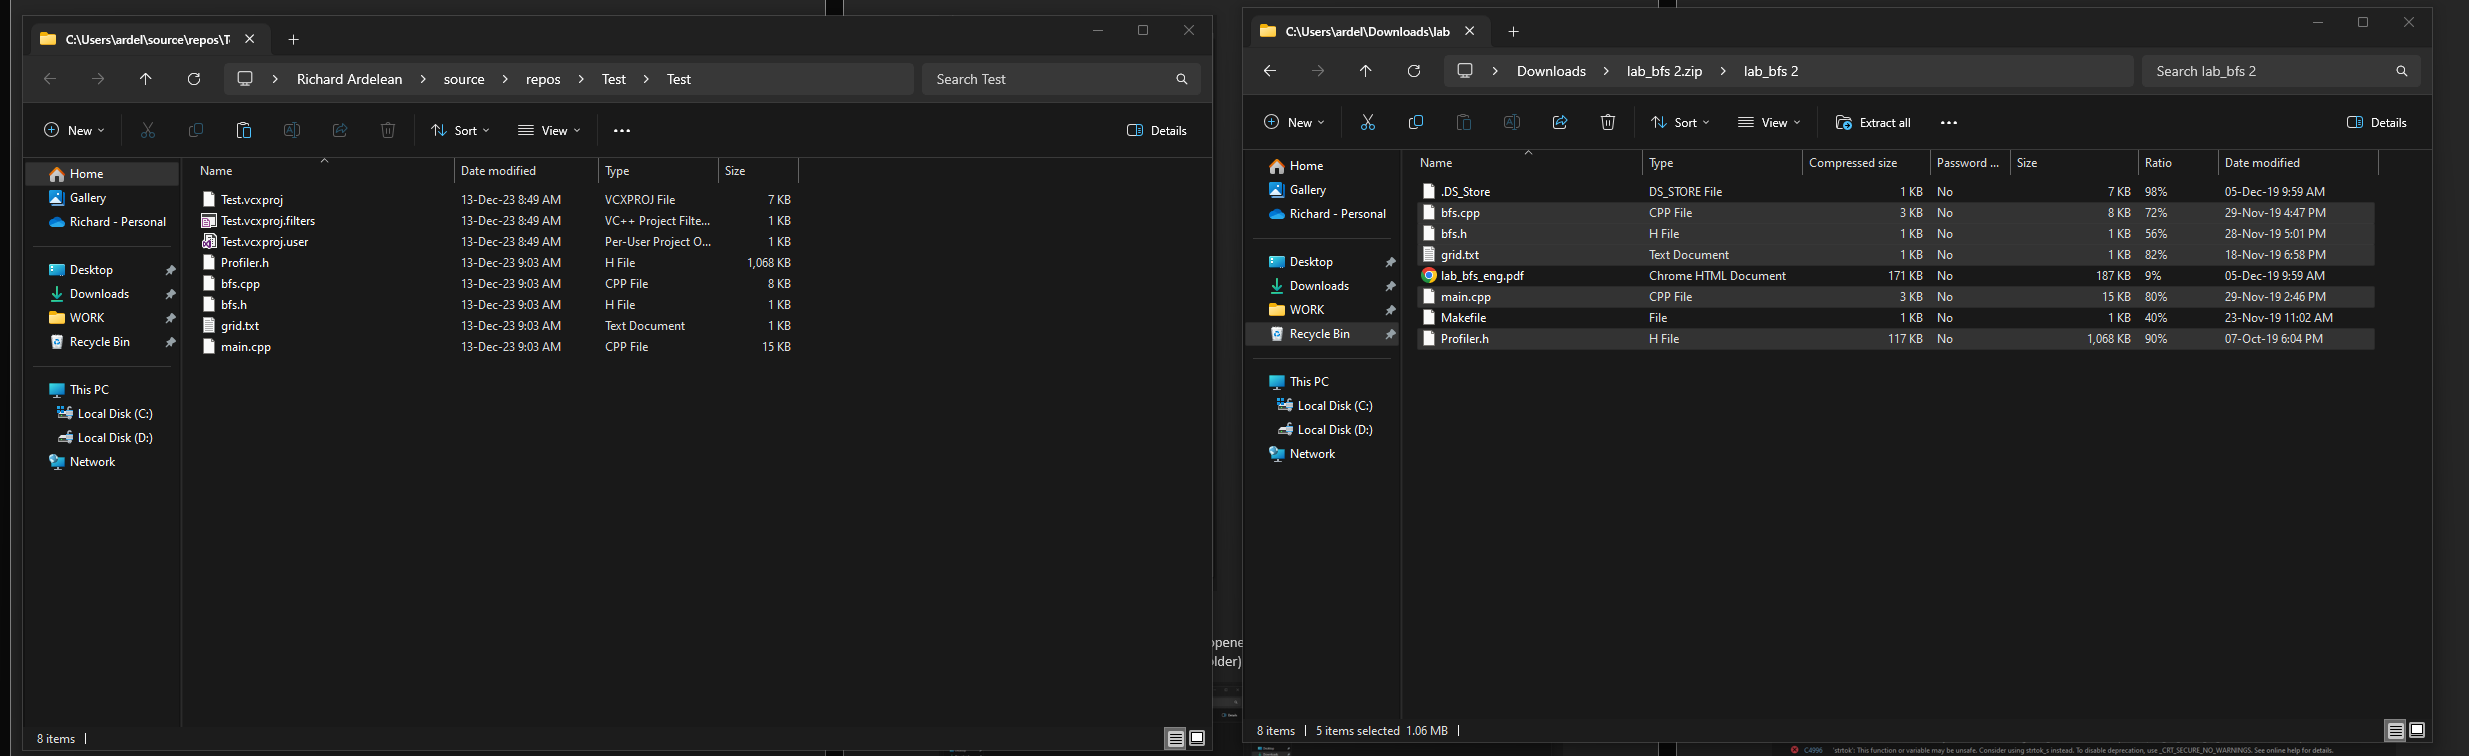
\includegraphics[width=\textwidth,alt={A screenshot of a computer Description automatically generated}]{./Resources/tutorial_lab9/image5.png}

\begin{enumerate}
\def\labelenumi{\arabic{enumi}.}
\setcounter{enumi}{4}
\item
  By selecting the folders from the Visual Studio Solution Explorer
  `Header Files / Resources / Source Files' use the following options:
\end{enumerate}

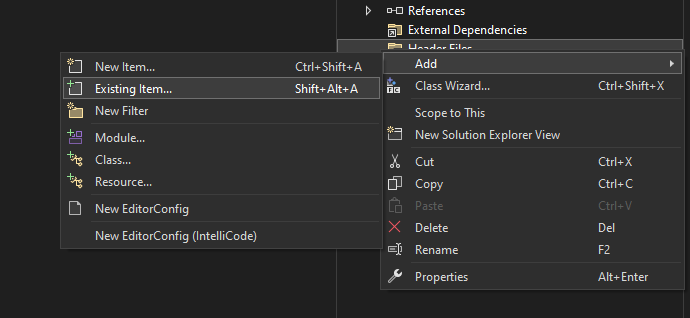
\includegraphics[width=\textwidth,alt={A screenshot of a computer Description automatically generated}]{./Resources/tutorial_lab9/image6.png}

\begin{enumerate}
\def\labelenumi{\arabic{enumi}.}
\setcounter{enumi}{5}
\item
  Such that, the following setup is accomplished:
\end{enumerate}

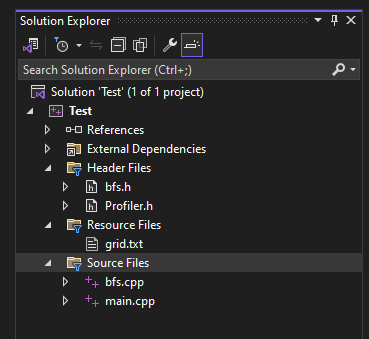
\includegraphics[width=\textwidth,alt={A screenshot of a computer Description automatically generated}]{./Resources/tutorial_lab9/image7.png}

\subsection{Visual Studio `unsafe' error}\label{visual-studio-unsafe-error}

Example:

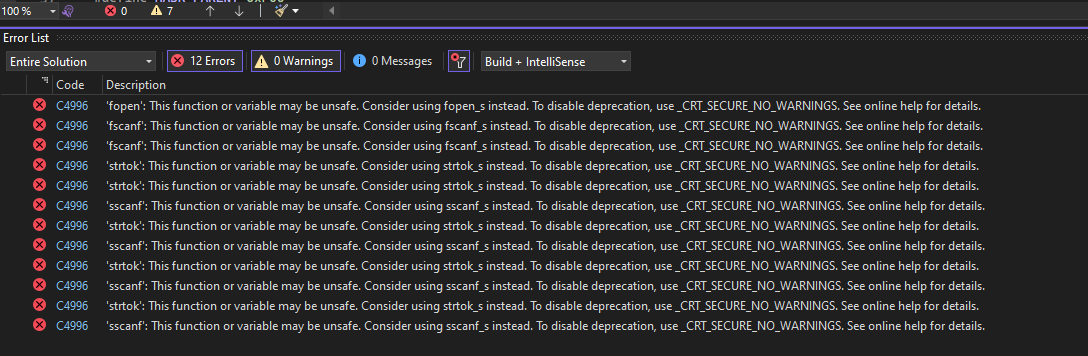
\includegraphics[width=\textwidth,alt={A screenshot of a computer Description automatically generated}]{./Resources/tutorial_lab9/image8.png}

Solution:

Right-click on the project (not the Solution which will most likely have
the same name) and select `Properties'.

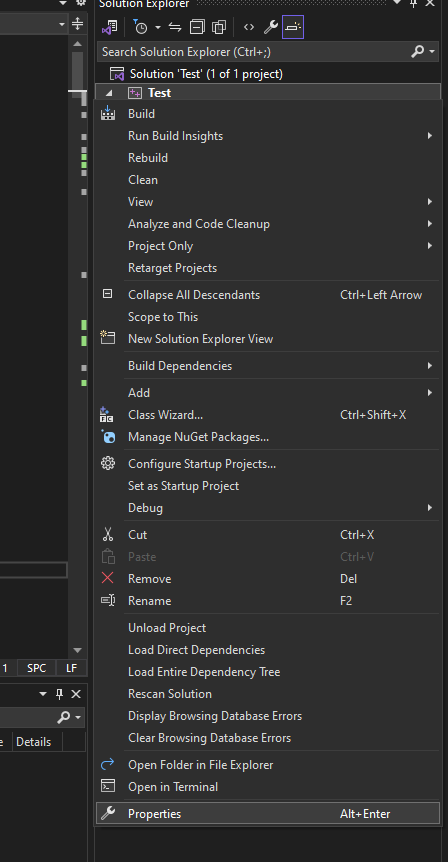
\includegraphics[width=\textwidth,alt={A screenshot of a computer program Description automatically generated}]{./Resources/tutorial_lab9/image9.png}

Update the `Configuration' and `Platform' in the upper side of the
window to `All Configurations' and `All Platforms', respectively.

Go to `C/C++' and select `Preprocessor'.

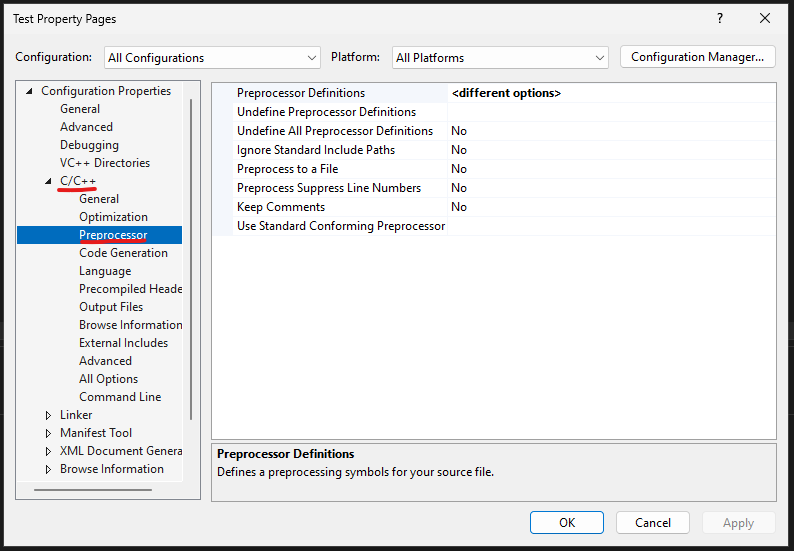
\includegraphics[width=\textwidth,alt={A screenshot of a computer Description automatically generated}]{./Resources/tutorial_lab9/image10.png}

Then click on `Preprocessor Definitions' and on the dropdown arrow.

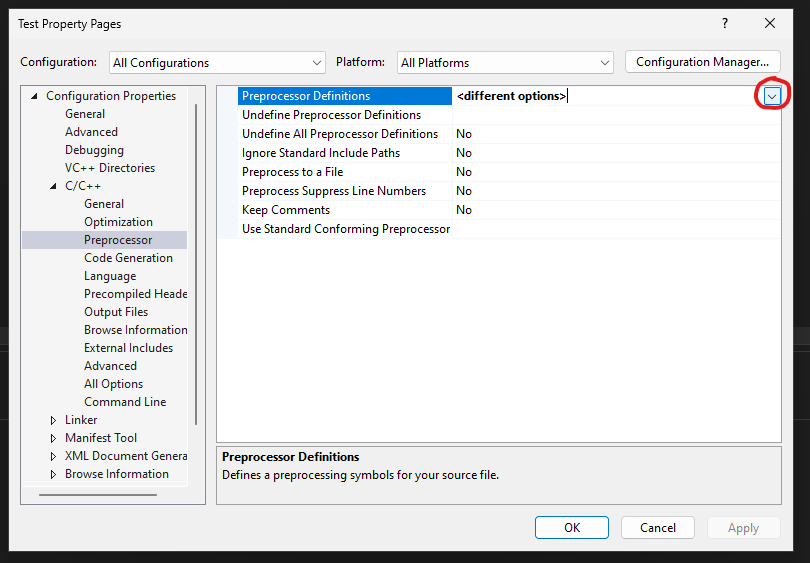
\includegraphics[width=\textwidth,alt={A screenshot of a computer Description automatically generated}]{./Resources/tutorial_lab9/image11.png}

Select `Edit'

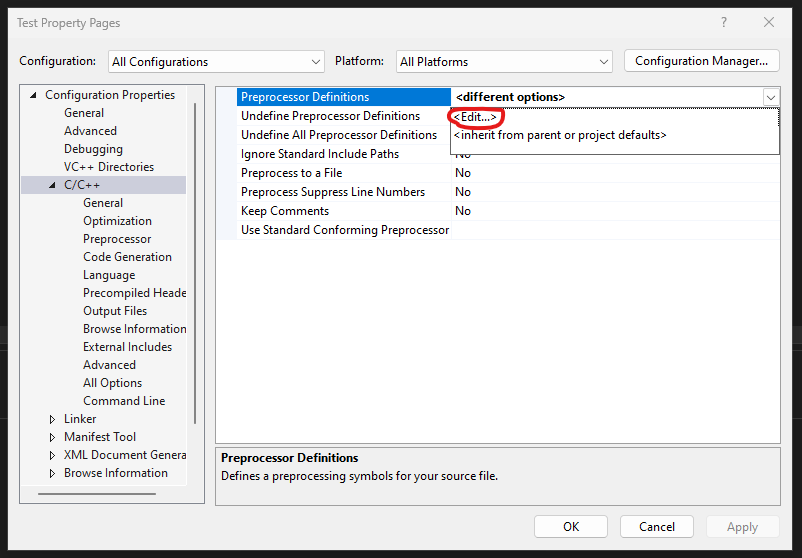
\includegraphics[width=\textwidth,alt={A screenshot of a computer Description automatically generated}]{./Resources/tutorial_lab9/image12.png}

And the following new window will open:

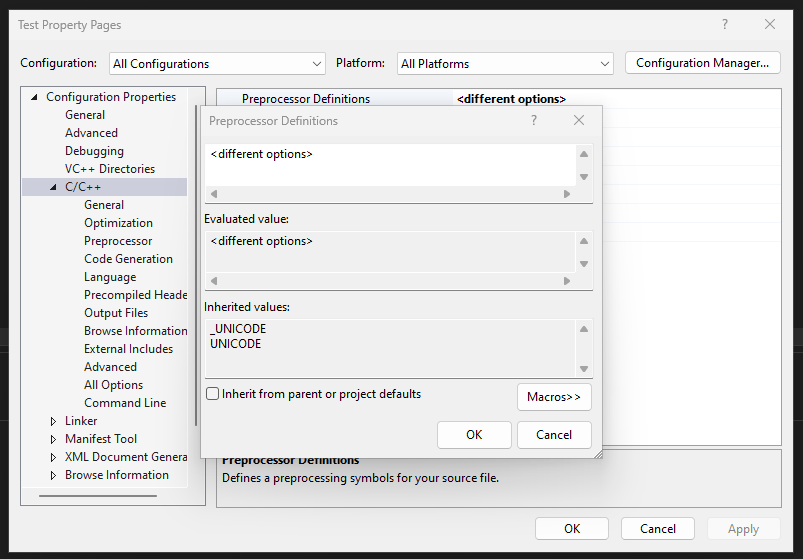
\includegraphics[width=\textwidth,alt={A screenshot of a computer Description automatically generated}]{./Resources/tutorial_lab9/image13.png}

Introduce `\_CRT\_SECURE\_NO\_WARNINGS' under `\textless different
options\textgreater' as shown below.

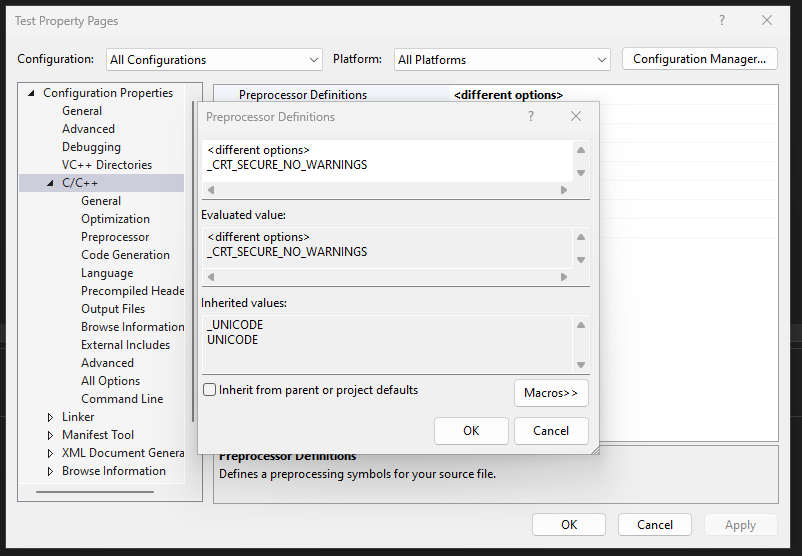
\includegraphics[width=\textwidth,alt={A screenshot of a computer Description automatically generated}]{./Resources/tutorial_lab9/image14.png}

Click on `OK' for all opened windows until you are returned to the main
Visual Studio window of the project, and you will be able to run the
project.

\subsection{Visual Studio `Assertion'
Error}\label{visual-studio-assertion-error}

This indicates that you have not followed the tutorial. Go back to the
first page and make sure that you have moved the files from the
`Downloads' folder to the `Project' folder. You might also need to
\emph{remove} all the files from the Visual Studio IDE and \emph{re-add}
them by hand.

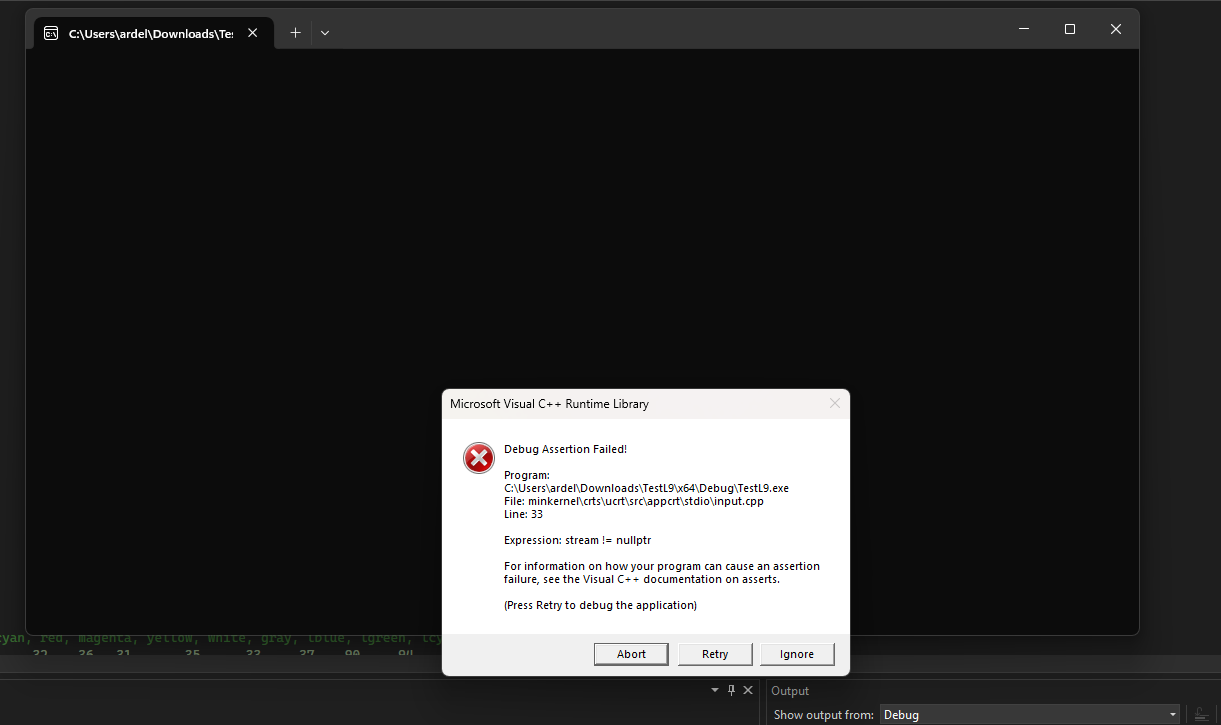
\includegraphics[width=\textwidth,alt={A screenshot of a computer Description automatically generated}]{./Resources/tutorial_lab9/image15.png}

\subsection{CLion undefined Error}\label{clion-undefined-error}

Example:

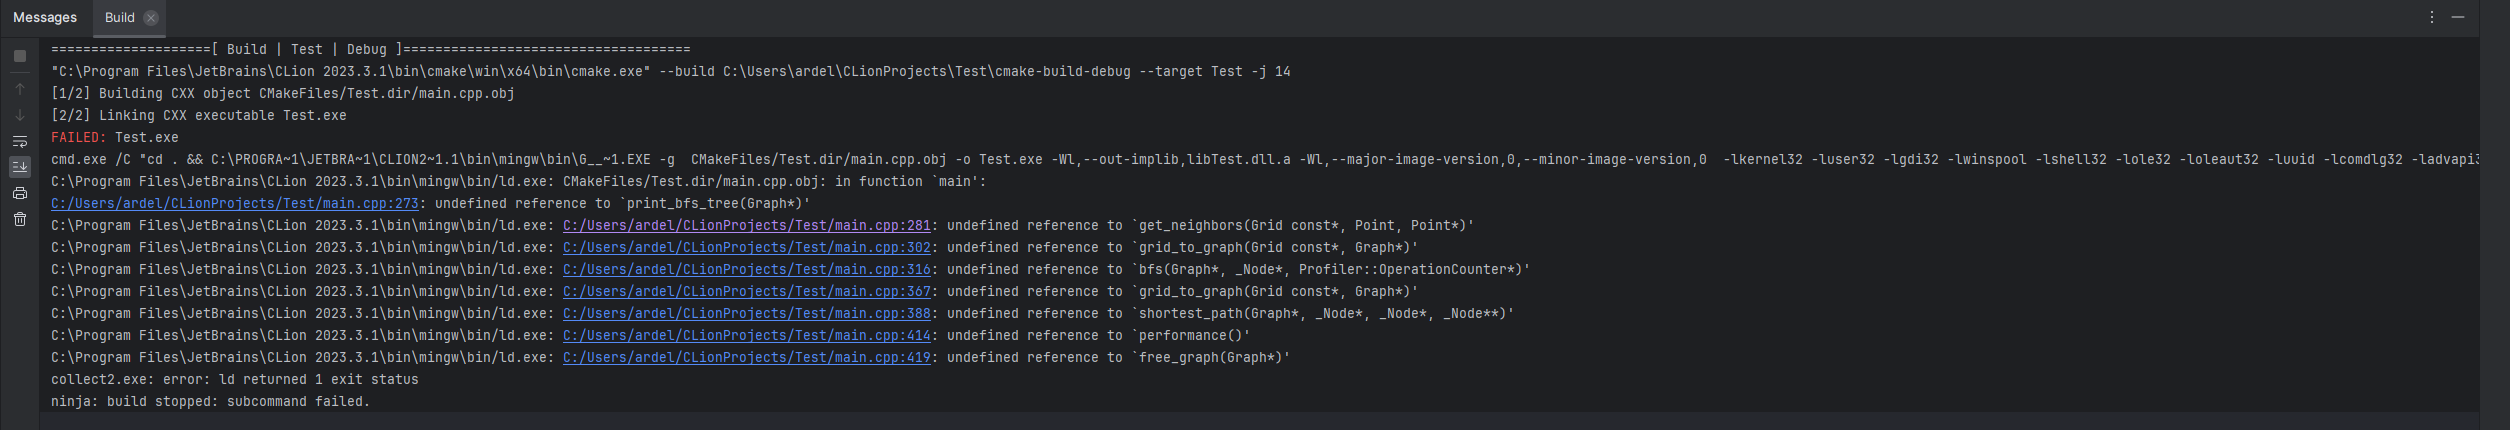
\includegraphics[width=\textwidth,alt={A screen shot of a computer Description automatically generated}]{./Resources/tutorial_lab9/image16.png}

Solution:

Open the `CMakeLists.txt' file and modify in the following manner:

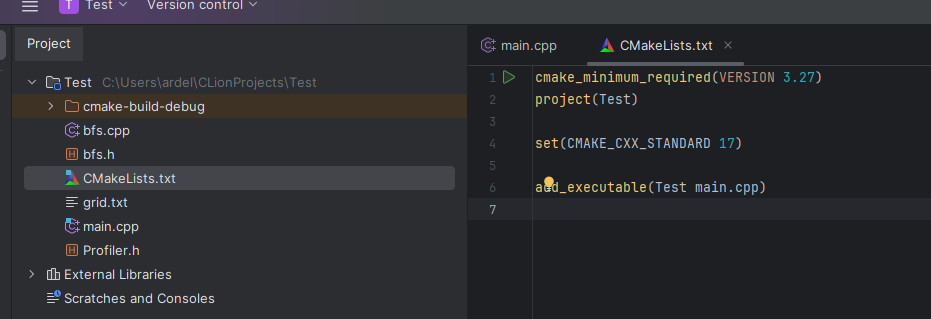
\includegraphics[width=\textwidth,alt={A screenshot of a computer Description automatically generated}]{./Resources/tutorial_lab9/image17.png}

add\_executable(Test main.cpp)

into

add\_executable(Test main.cpp bfs.cpp)

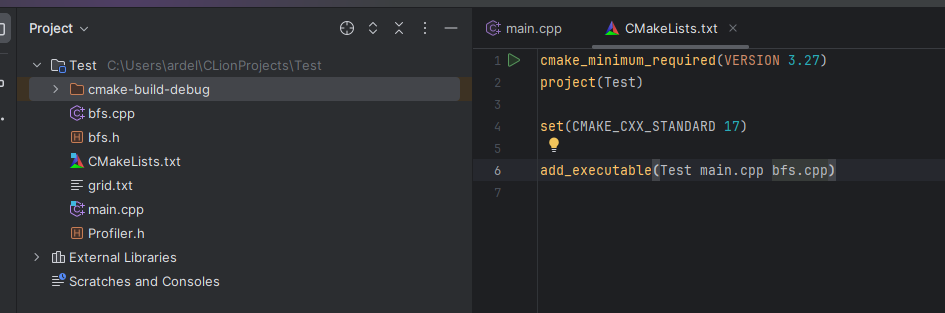
\includegraphics[width=\textwidth,alt={A screenshot of a computer Description automatically generated}]{./Resources/tutorial_lab9/image18.png}

\subsection{CLion Visual Studio -- Option 1
(slower)}\label{clion-visual-studio-option-1-slower}

Go to File -\textgreater{} Settings:

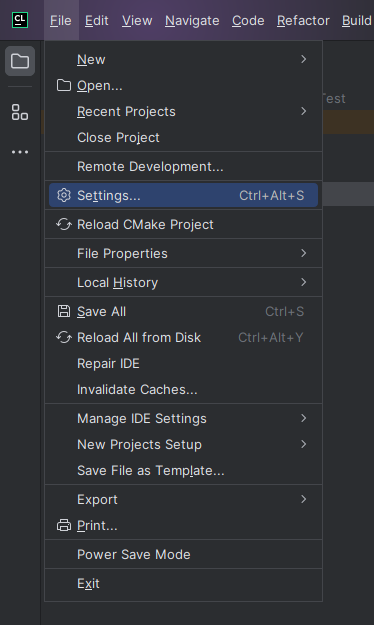
\includegraphics[width=\textwidth,alt={A screenshot of a computer program Description automatically generated}]{./Resources/tutorial_lab9/image19.png}

In the newly opened window, go to `Build, Execution, Deployment'
-\textgreater{} `Toolchains'

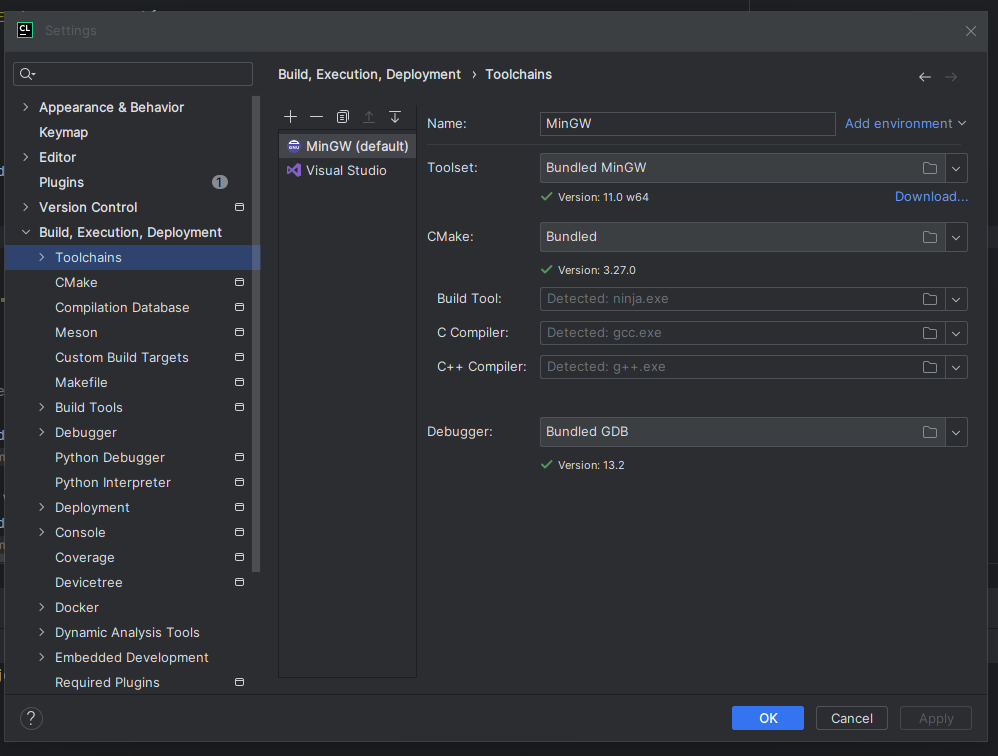
\includegraphics[width=\textwidth,alt={A screenshot of a computer Description automatically generated}]{./Resources/tutorial_lab9/image20.png}

Using the arrows, move Visual Studio as default:

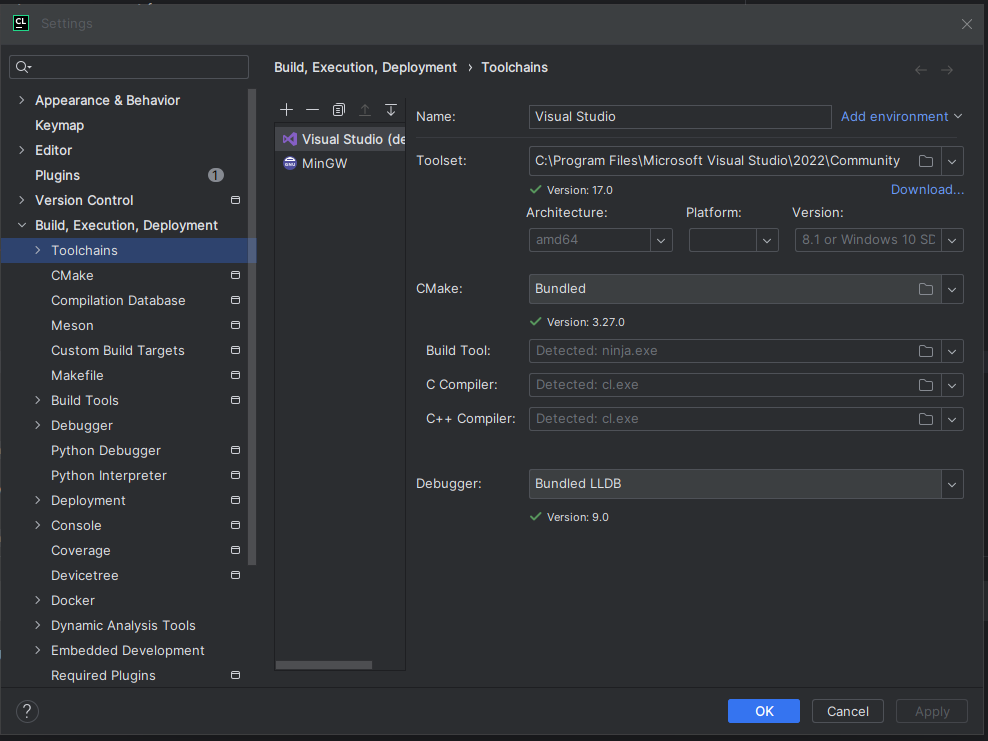
\includegraphics[width=\textwidth,alt={A screenshot of a computer Description automatically generated}]{./Resources/tutorial_lab9/image21.png}

\subsection{CLion MinGW -- Option 2 (faster, requires external
console)}\label{clion-mingw-option-2-faster-requires-external-console}

\subsubsection{\texorpdfstring{CLion Clear error
}{CLion Clear error }}\label{clion-clear-error}

Example:

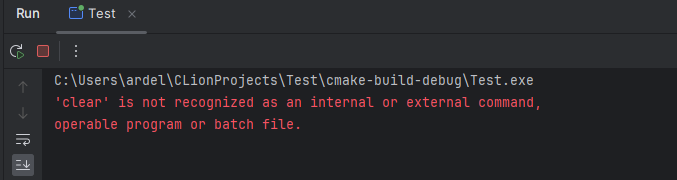
\includegraphics[width=\textwidth,alt={A screenshot of a computer program Description automatically generated}]{./Resources/tutorial_lab9/image22.png}

Solution:

Go to the main.cpp file and scroll to lines 113-117 in the displayGrid
function.

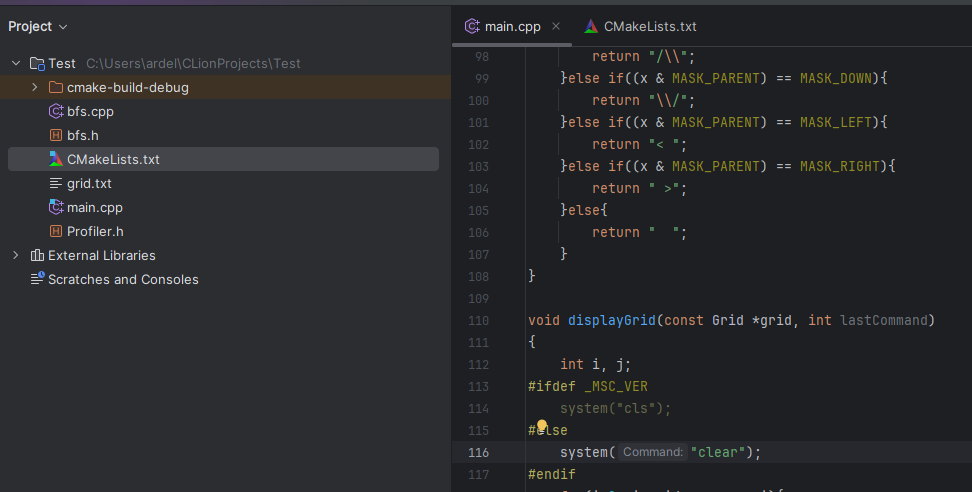
\includegraphics[width=\textwidth,alt={A screen shot of a computer Description automatically generated}]{./Resources/tutorial_lab9/image23.png}

Modify in the following manner:

In the else branch from line 116

system("clear");

to

system("cls");

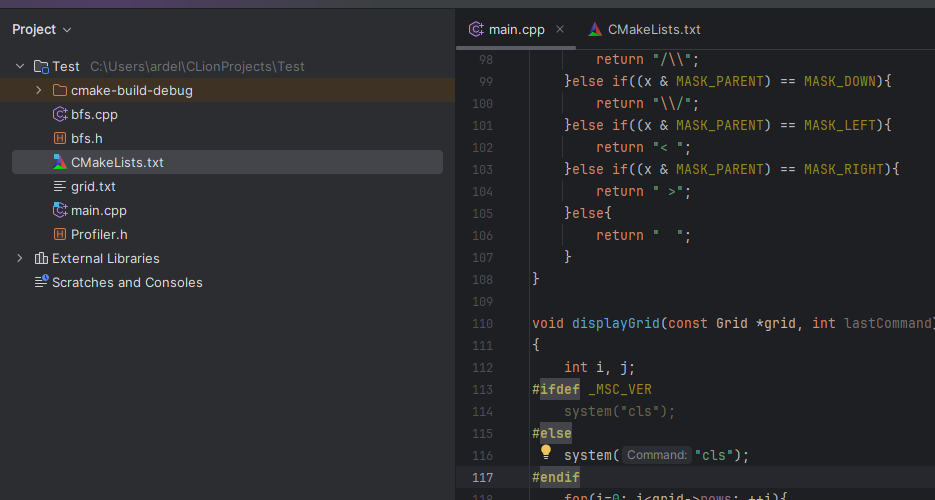
\includegraphics[width=\textwidth,alt={A screenshot of a computer program Description automatically generated}]{./Resources/tutorial_lab9/image24.png}

\subsubsection{CLion not showing grid}\label{clion-not-showing-grid}

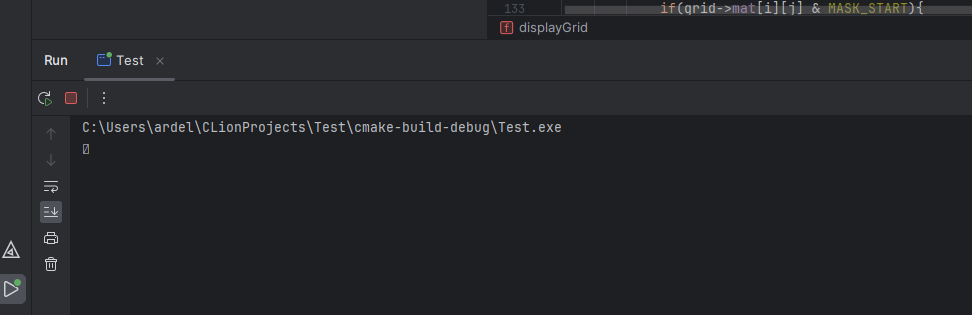
\includegraphics[width=\textwidth,alt={A screenshot of a computer Description automatically generated}]{./Resources/tutorial_lab9/image25.png}

Copy the `grid.txt' file into the `cmake-build-debug' folder.

Then go to the upper right part of the screen:

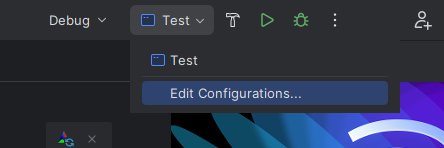
\includegraphics[width=\textwidth,alt={A screenshot of a computer Description automatically generated}]{./Resources/tutorial_lab9/image26.png}

Select `Edit Configurations' and check the following boxes:

\begin{itemize}
\item
  Run in external console
\end{itemize}

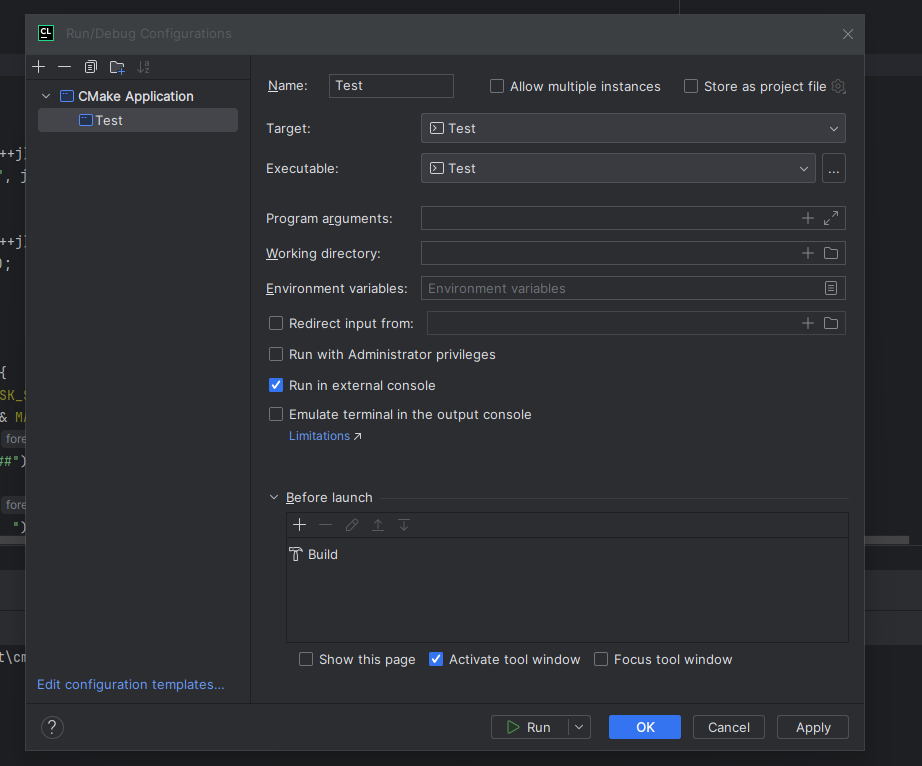
\includegraphics[width=\textwidth,alt={A screenshot of a computer Description automatically generated}]{./Resources/tutorial_lab9/image27.png}

\subsection{Mac run command}\label{mac-run-command}

g++ main.cpp bfs.cpp -std=c++11 \&\& ./a.out


\end{document}